%!TEX root = ../artigo.tex
\section{Sintelo} % (fold)
\label{sec:sintelo}
A ferramenta sintelo é uma ferramenta didática para o ensino de compiladores. A mesma foi criada por Karina Kieling Dos Santos e Philipe Marcon Dos Reis, no ano de 2008 como Trabalho de Conclusão de Curso pela Universidade
do Sul de Santa Catarina e foi publicada em \cite{sintelo}. 

Embora a ferramenta em questão possua mais funcionalidades, esse trabalho se limitou a parte de análise léxica, permanecendo em seu escopo.

Para que possamos realizar a análise léxica, primeiramente devemos informar ao sintelo os tokens de nossa linguagem, através de expressões regulares. Essas expressões regulares devem ser informadas na ``caixa'' chamada léxico, conforme ilustrado na figura~\ref{sintelo-inicial}.

\begin{figure}[ht!]
	\centering
	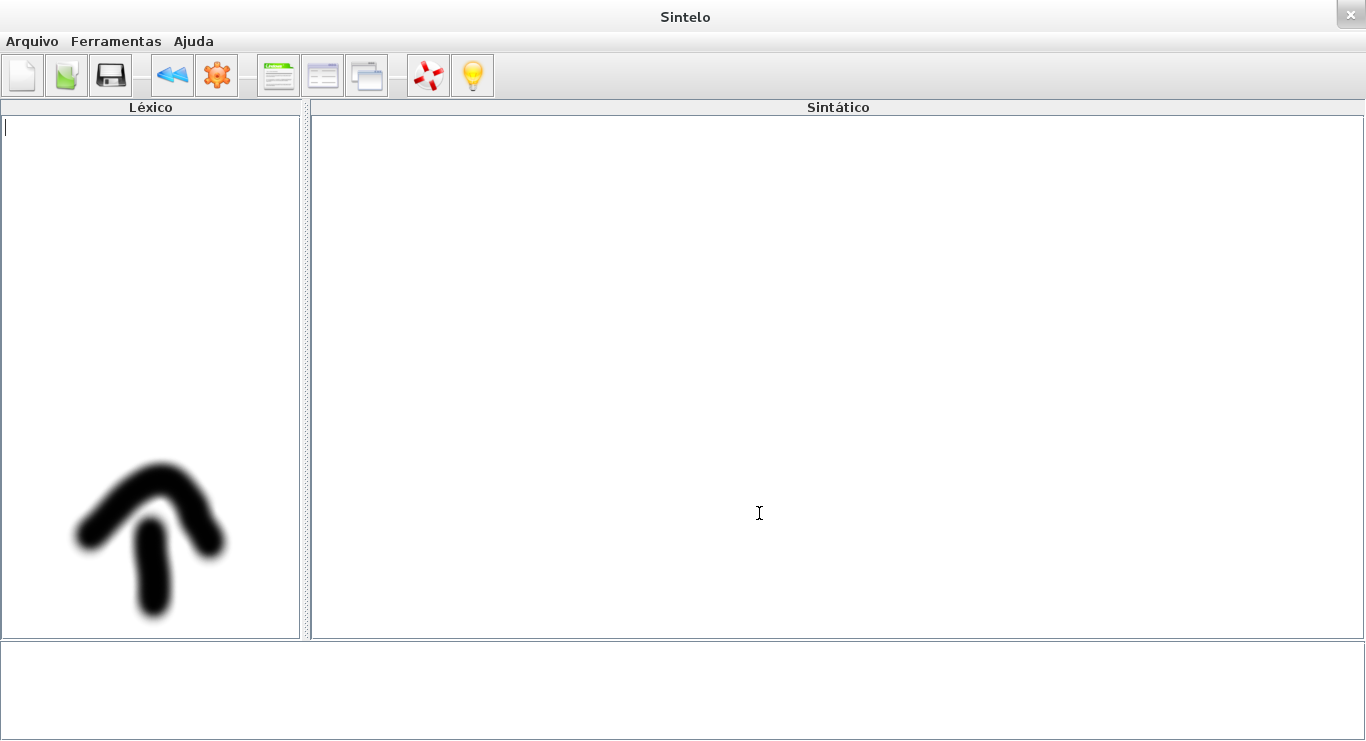
\includegraphics[scale=0.28]{imgs/sintelo-inicial-ed}
	\caption{Tela inicial do sintelo.}
	\label{sintelo-inicial}
\end{figure}

A notação utilizada para representar as expressões regulares são descritas em \cite{sintelo} ou no manual da ferramenta, que pode ser acessado através do menu ``Ajuda'', item ``Manual'' e seção ``Especificações Léxicas''. Desta forma este artigo não explicará a notação.

\subsection{Exemplo} % (fold)
\label{sub:exemplo}
Para exibir a análise léxica, o exemplo de operações aritméticas de \cite{Sebesta201201} será adaptado. Esse exemplo reconhece operações aritméticas que podem conter números (inteiros e/ou reias), identificadores (variáveis), operações binárias e também parêntesis; ignorando espaços em branco, quebra de linha e tabulação.

A seguir, a especificação dos tokens que deve ser passada para o sintelo:
\begin{verbatim}
ID:[a-zA-Z_][_a-zA-Z0-9]*
INT:[0-9]+
REAL:([0-9]\.[0-9]+) | ([0-9]+\.[0-9])
"("
")"
binop:"+" | \- | \*|"/"
:[\s\n\t]+
\end{verbatim}

Com os tokens da linguagem especificados, basta realizar a simulação da análise léxica. Para fazer isso, primeiramente vá ao menu ``Ferramentas'', item ``Léxico'', opção ``Simular''. 

\begin{figure}[ht!]
	\centering
	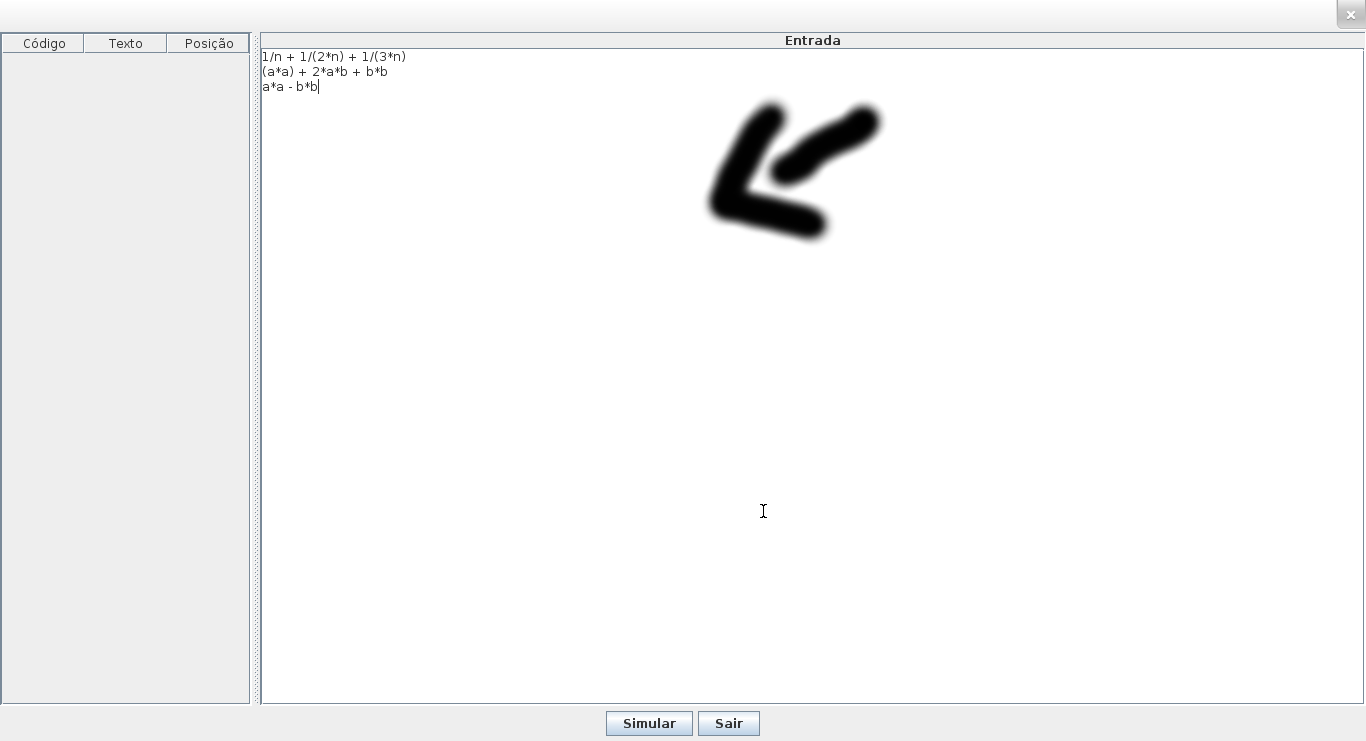
\includegraphics[scale=0.28]{imgs/sintelo-lexico-inicial}
	\caption{Tela inicial da simulação da análise léxica.}
	\label{sintelo-lexico-inicial}
\end{figure}

A seguir, é necessário informar a entrada da linguagem, no local informado pela figura ~\ref{sintelo-lexico-inicial}. Como exemplo de entrada para o analizador léxico, temos a seguinte:
\begin{verbatim}
1/n + 1/(2*n) + 1/(3*n)
(a*a) + 2*a*b + b*b
a*a - b*b
\end{verbatim}

Para efetuar a simulação basta clicar no botão ``Simular''. A figura ~\ref{sintelo-lexico-ok} exibe o resultado da simulação. Note que a ferramenta exibe os tokens reconhecidos e seus respectivos lugares no código de entrada.
\begin{figure}[ht!]
	\centering
	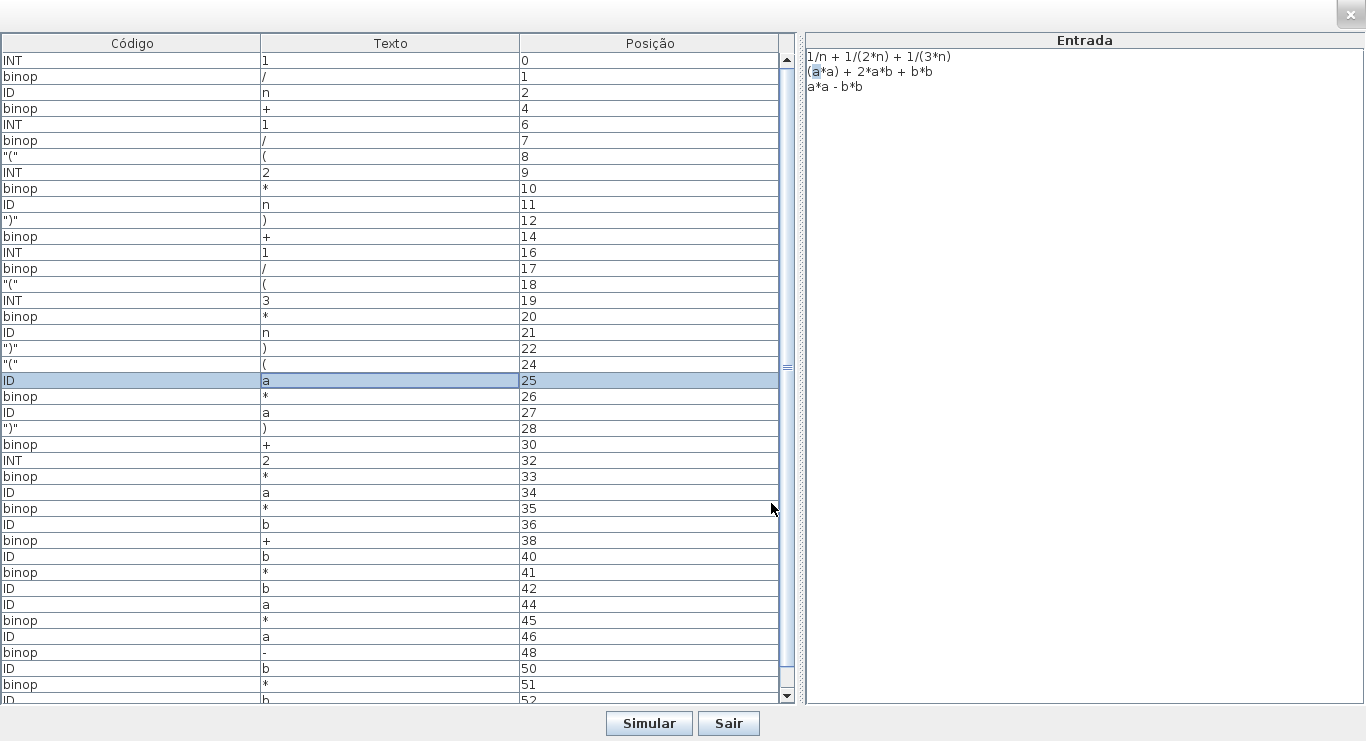
\includegraphics[scale=0.28]{imgs/sintelo-lexico-ok}
	\caption{Tela após a simulação da análise léxica.}
	\label{sintelo-lexico-ok}
\end{figure}

Agora considere a seguinte entrada:
\begin{verbatim}
a^a - b*b
\end{verbatim}

Como a operação \^~ não está definida na linguagem em questão, um erro será obtido com a simulação dessa entrada, conforme ilustrado na figura ~\ref{sintelo-lexico-erro}. 

\begin{figure}[ht!]
	\centering
	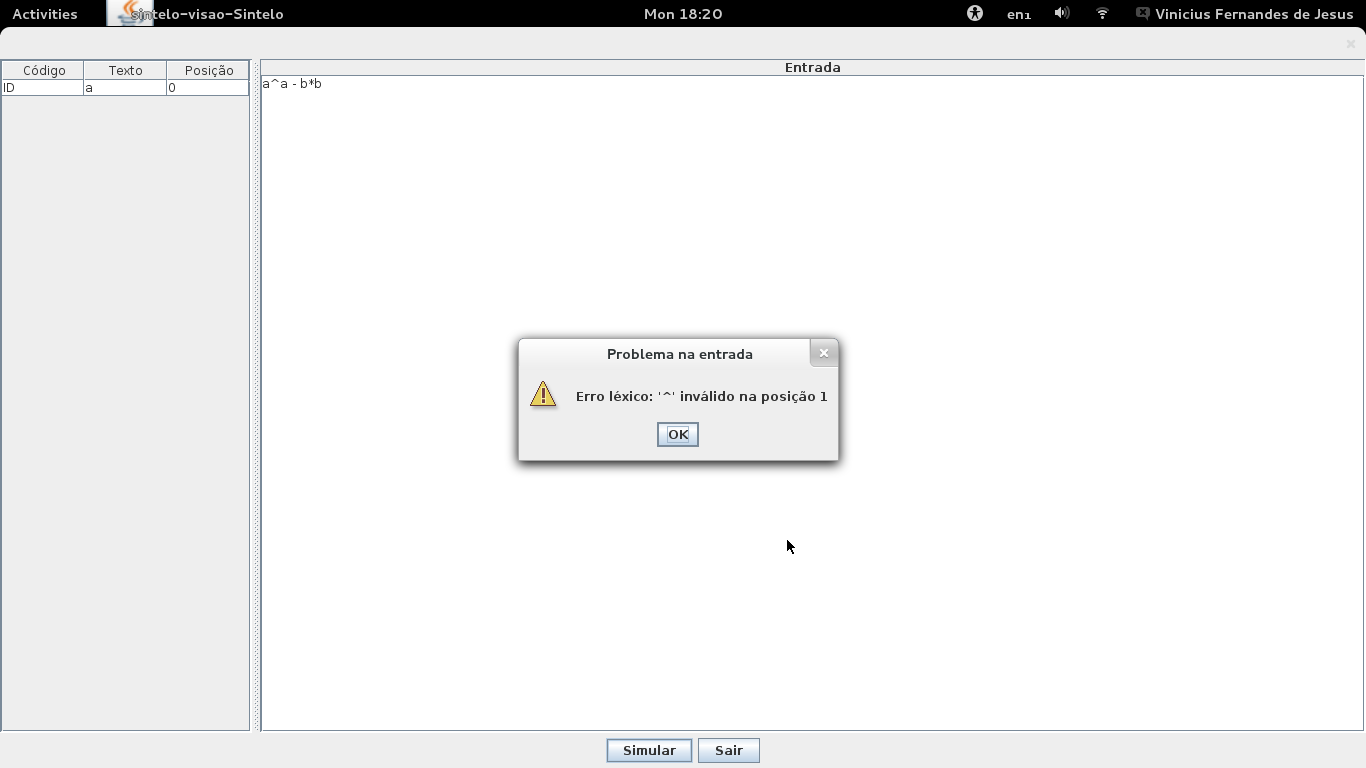
\includegraphics[scale=0.28]{imgs/sintelo-lexico-erro}
	\caption{Tela de erro léxico.}
	\label{sintelo-lexico-erro}
\end{figure}

No sintelo, também podemos visualizar o autômato gerado a partir das expressões regulares. Basta ir ao menu ``Ferramentas'', item ``Léxico'', opção ``Tabela de Transição''. A figura \ref{sintelo-lexico-automatan} ilustra o automato do exemplo utilizado.

\begin{figure}[ht!]
	\centering
	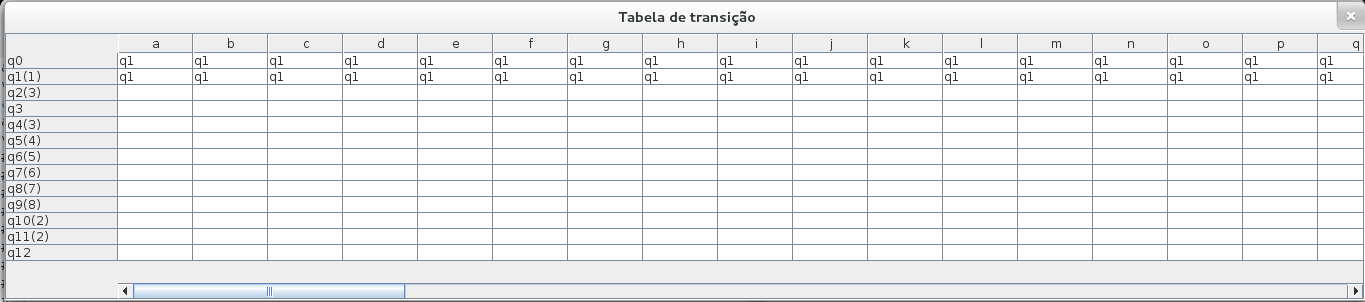
\includegraphics[scale=0.28]{imgs/sintelo-lexico-automatan}
	\caption{Automato do exemplo em questão.}
	\label{sintelo-lexico-automatan}
\end{figure}
% subsection exemplo (end)

\subsection{Considerações} % (fold)
\label{sub:consideracoes}
O sintelo é uma boa ferramenta educativa, possuindo uma boa interface com o usuário. O único problema dessa interface é que seu editor não possui funcionalidades que ajudam a formar os tokens, como opção de voltar, multiplas seleções, etc.

Além do mais, essa ferramente é muito fácil de se utilizar, visto que seu manual contém todas as informações necessárias e que todos os erros são corretamente informados para o usuário. Desta forma, o Sintelo é uma ótima ferramenta para auxiliar o ensino da disciplina de compiladores.

No entento, por ser de carater educativo, há uma certa dificuldade em realizar a análise léxica de uma linguagem real completa, como C/C++.

\begin{table}[ht]
\caption{Considerações do Sintelo}
\centering
\begin{tabular}{|m{1.6cm}|m{1.5cm}|m{1.5cm}|m{1.5cm}|m{1.5cm}|m{1.8cm}|m{1.5cm}|}  \hline
   Ferramenta & Design da interface com o usuário & Facilidade de uso da ferramenta & Interação com o usuário & Facilidade de aplicação da fundamentação teórica & Capacidade de aplicação das ramificações teóricas & Relação entre uso e aprendizado \\ \hline
Sintelo & Bom & Ótimo & Ótimo &  Bom & Bom & Ótimo \\ \hline
\end{tabular}
\label{table:caracteristicas_sintelo}
\end{table}

% subsection consideracoes (end)

% section sintelo (end)